\section{Komponenten}

\subsection{Physische Komponenten}

\subsubsection{Intel RealSense D435}

\begin{figure}[H]
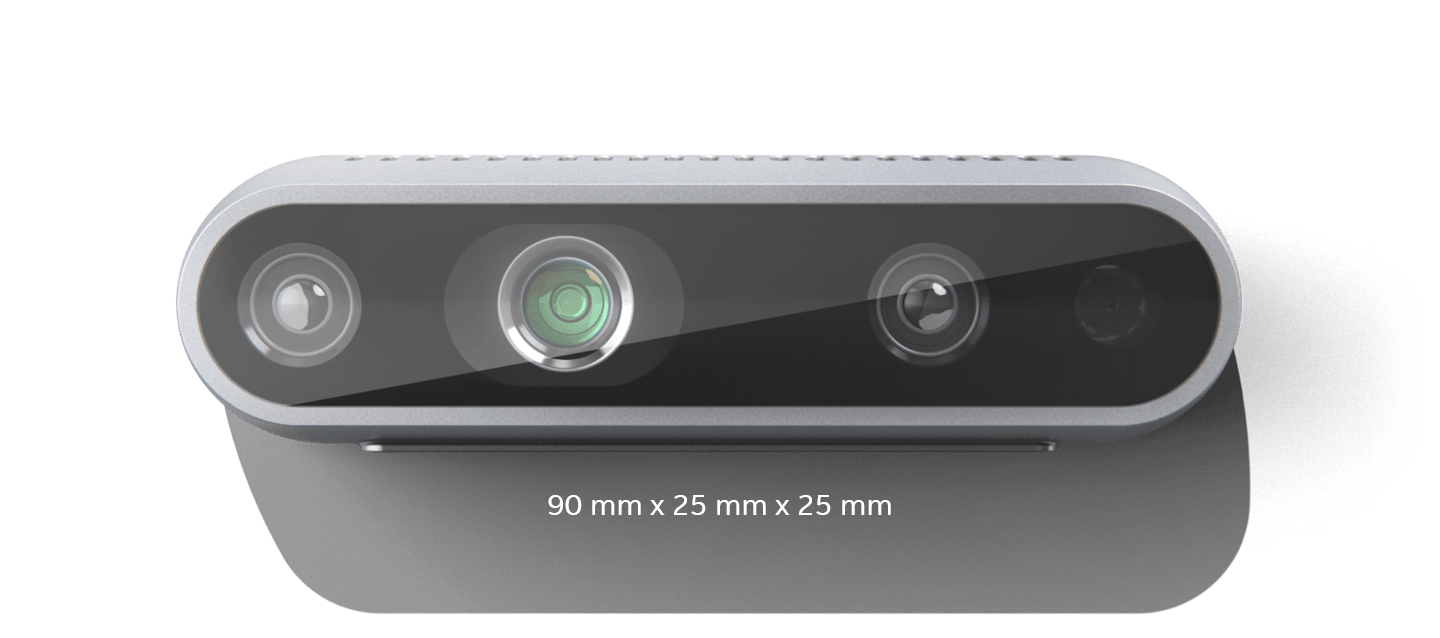
\includegraphics[width=0.6\linewidth]{435d}
\caption{Intel RealSense D435, Frontside}
\label{fig:D435:1}
\end{figure}


Die Kamera IntelRealSense D435 von Intel hat ein breites Sichtfeld, einen globalen Shutter und einen Tiefensensor, der sich für Anwendungen mit schnellen Bewegungen eignet. Gerade durch ihr breites Sichtfeld eignet sich die Kamera für Anwendungen in der Robotik, Virtual und Augmented Reality, bei Szenen wo es darum geht möglichst viel zu sehen. Sie hat eine Reichweite bis zu 10 Meter. Das Intel RealSenseSDK bietet plattformunabhängig Unterstüzung bei der Umsetzung.
Für mein Projekt sollte diese Kamera also genügen. Wie gross das Sichtfeld dann wirklich ist, wird sich zeigen.
			
\begin{figure}[H]
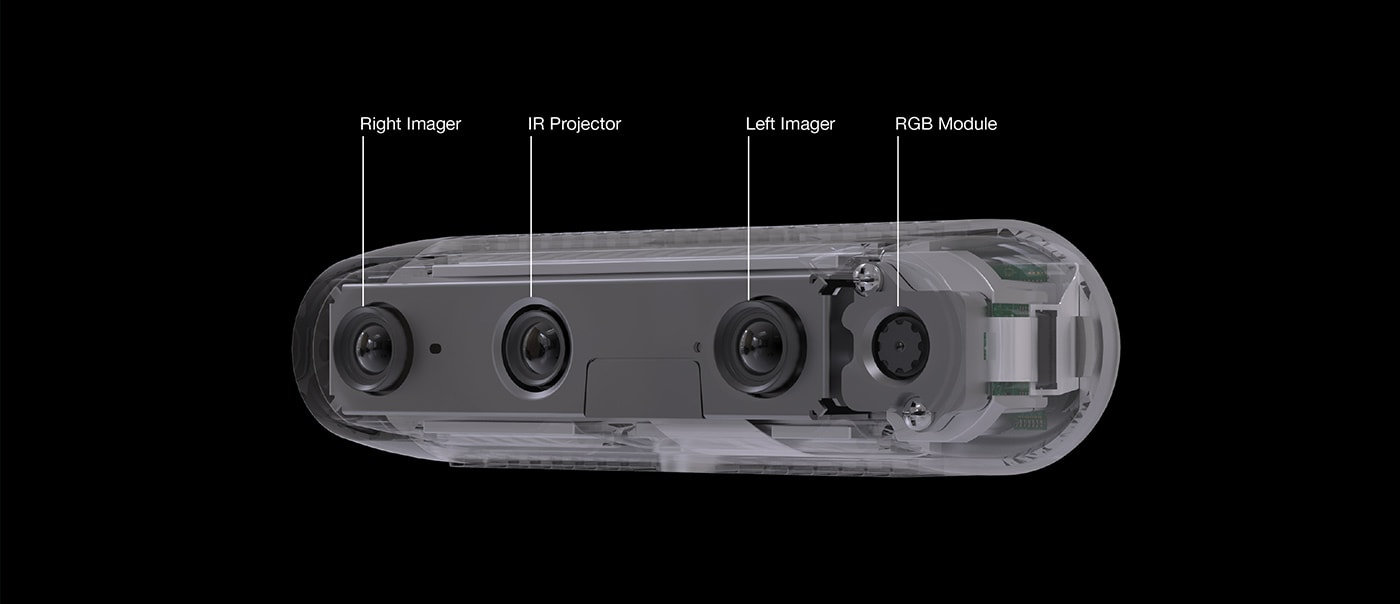
\includegraphics[width=0.6\linewidth]{435d_back}
\caption{Intel RealSense D435, Backside}
\label{fig:D435:2}
\end{figure}
			
Die Global-Shutter-Sensoren haben eine hohe Lichtempfindlichkeit bei schlechten Lichtverhältnissen und ermöglichen die Steuerung von Robotern auch in dunklen Räumen.
\cite{Intel} \\
Die Lichtverhältnisse in einem Raum der künstlich beleuchtet werden kann, spielen in meinem Projekt eine untergeordnete Rolle. Wichtig ist eigentlich nur, dass diese Tiefenkamera die getrackten Positionen richtig erfasst und möglichst in Realtime updatet.

\subsection{Software Komponenten}

\subsubsection{Intel RealSense Viewer}

Der Intel RealSense Viewer hat zwei Frames die er anzeigen kann, den RGB Frame und den Depth Frame. Die Abbildung zeigt einen Screenshot vom Depth Frame.

\begin{figure}[H]
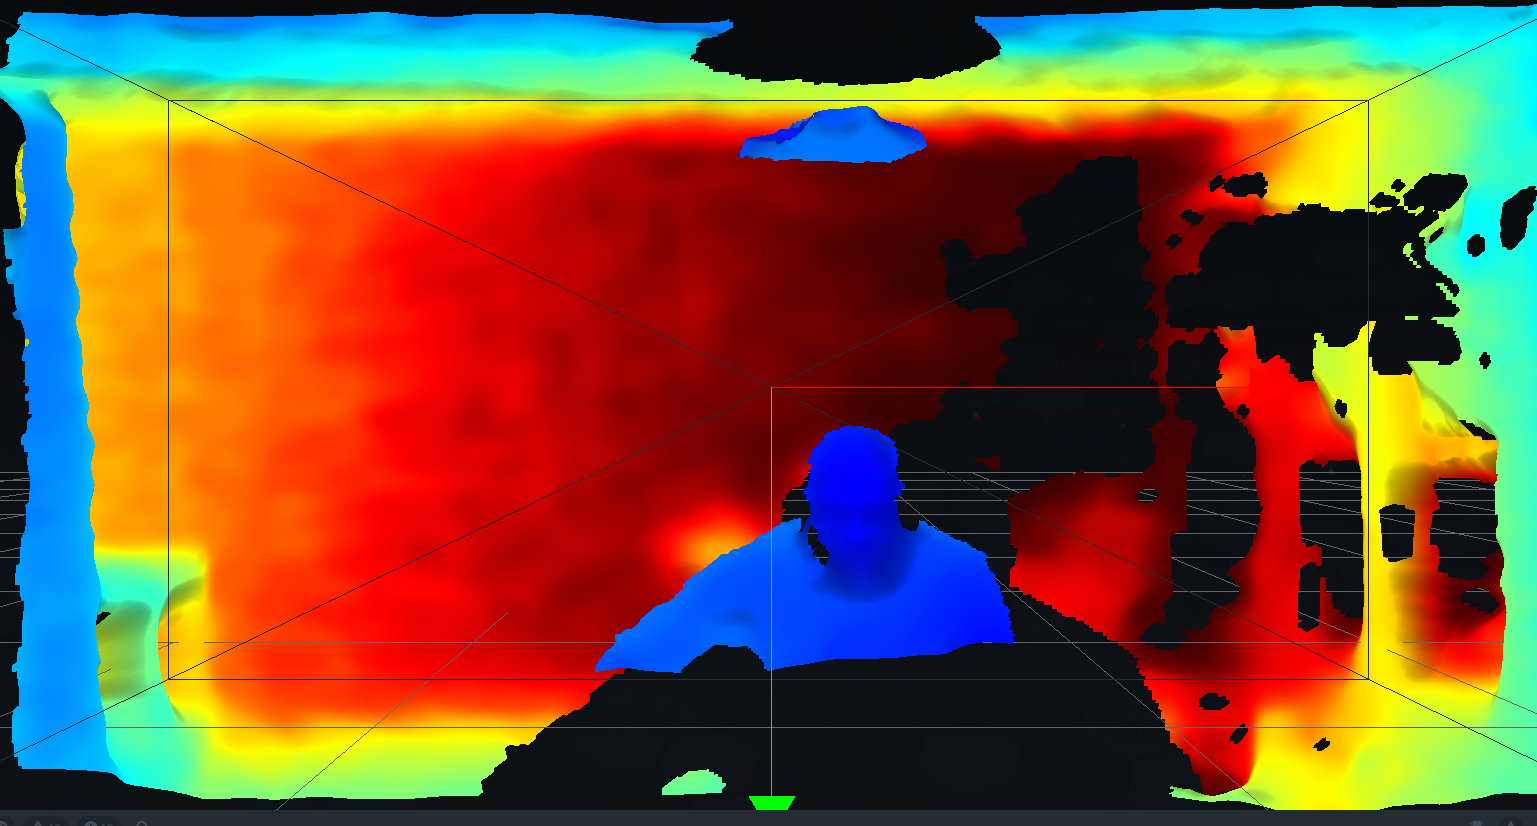
\includegraphics[width=0.6\linewidth]{depth_sensor}
\caption{Intel RealSense Viewer, Depth Frame}
\label{fig:RealSense Viewer}
\end{figure}
		
Die blauen Farbpixel zeigen einen nahen Bildpunkt, die roten Farbpixel einen entfernten Bildpunkt. \\ Für mein Projekt eignent sich dieser Viewer einzig dazu die verschiedenen Kameraeinstellungen auszuprobieren.
			
\subsubsection{Intel RealSenseSDK 2.0}

Intel hatte vor einigen Jahren eine führende Rolle in Anwendungen im Bereich Augmented Reality. Mit dem Intel RealSenseSDK 2016, dem Vorgänger vom RealSenseSDK 2.0 gab es ein ToolKit, welches Facetracking implementiert hatte. Die rechte und die linke Hand konnten beispielsweise seperat fürs Tracking angesteuert werden und mehr noch: Sogar einzelne Finger einer Hand konnten getrackt werden. \\ Ich habe noch versucht dieses ältere SDK zu installieren und dann mit einer älteren Unity Version zu verwenden. Leider ohne Erfolg. Intel hatte eine ganze Videoreihe dazu erstellt, welche aber heute vom Netz genommen wurde.\\
Intel schließt seine Abteilung rund um die RealSense-Kameras, die viele Jahre interessante, aber vom Markt kaum umgesetzte Lösungen hervorgebracht hatte. Sie passt nicht zum neuen Geschäftsmodell, welches rund um die Kernthemen von Intel aufgebaut und von dem neuen Foundry-Geschäft unterstützt wird.
\cite{ComputerBase} \\ Das neue SDK 2.0 taugt dagegen nur noch wenig und eignet sich nicht für mein Projekt. Das Toolkit implementiert kein Facedetection mehr. \\ Eigentlich sehr Schade, das aufgebaute Know-How still zu legen.

\subsubsection{Unity}

Unity ist eine Game Engine die von einer Open Source Community betreut und weiterentwickelt wird. \cite{Unity} \\ Unity bietet für dieses Projekt ein anwendungsfreundliches Toll mit welchem die virtuelle Szene dargestellt werden kann. In Unity können viele Plugins installiert werden, die mir dann auch sehr nützlich sein werden. Ein weiterer Vorteil von Unity ist die grosse Community und die vielen Beiträge wie Probleme gelöst werden können. 

			
			
\subsubsection{Nuitrack}
Nuitrack ist eine Tracking Software, die viel mehr kann, als ich für dieses Projekt benötige. \\
Nuitrack stellt in ihrem SDK viele Anwendungen zur Verfügung, diese sind aber auf 3 Minuten Spieldauer limitiert. Wahrscheinlich haben sie von Intel gelernt und haben ein Pricing welches für volle Anwendungen \$99.99 pro Jahr kostet. In der nächsten Abbildung sind alle implementierten Features dargestellt.

\begin{figure}[H]
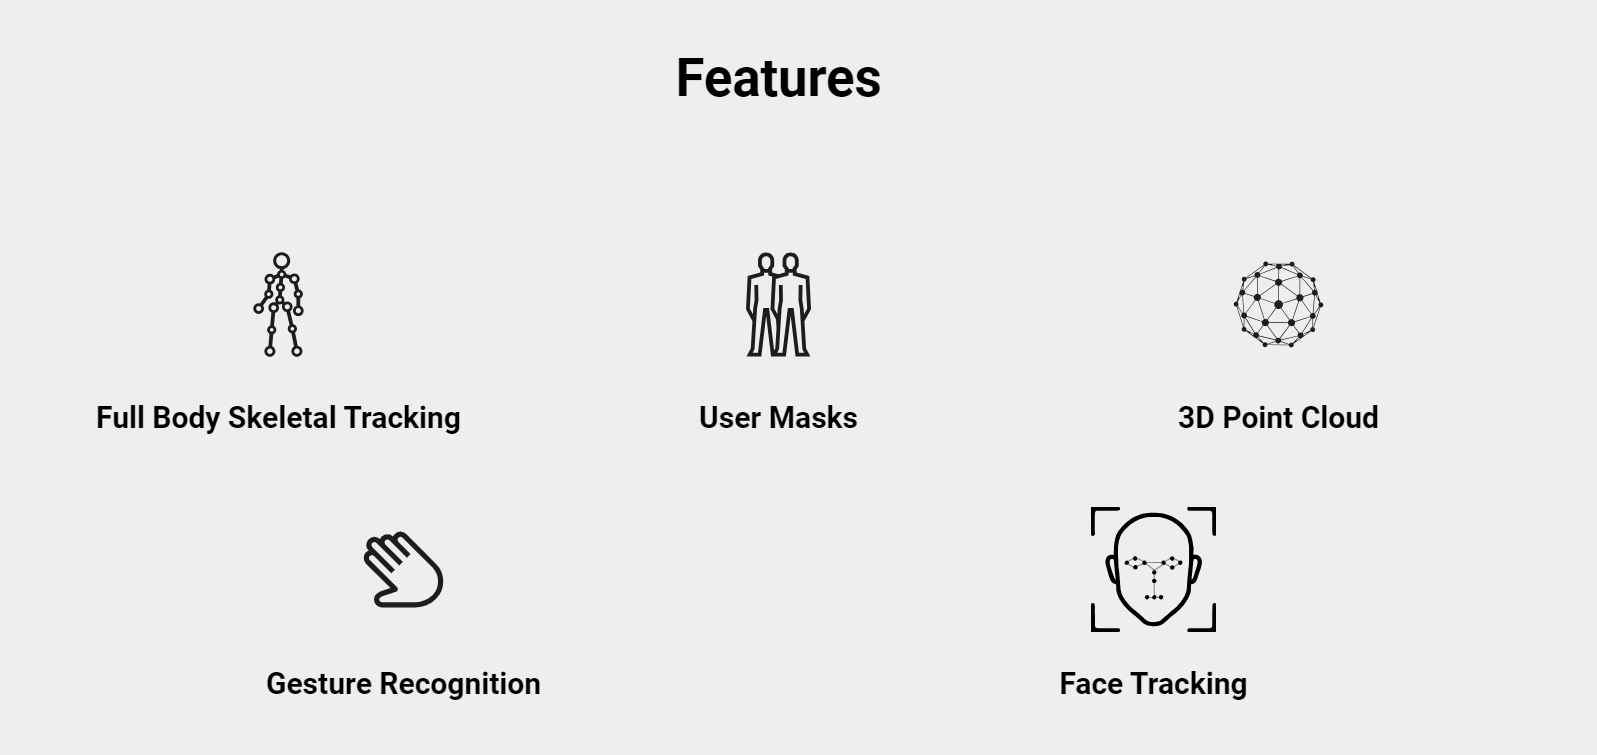
\includegraphics[width=1.0\linewidth]{nuitrack_features}
\caption{Nutitrack SDK, Features}
\label{fig:Nuitrack Features}
\end{figure}

Dieses SDK ist enorm mächtig und hat alles zu bieten, was ich für mein Projekt brauche. Wichtig für mein Projekt ist das Facetracking und das Full Body Skeletal Tracking. Die Nutirack SDK hat eine gute Anbindung zu Unity und ist gut dokumentiert.
\cite{NuitrackSDK} 

\subsection{OpenCV}

OpenCV ist eine Open Source Computer Vision Grafik Library. In meinem Projekt benötige ich diese Library um ein bliebiges Polygon mit- vier Seiten zu entzerren und als Rechteck darzustellen. Es gibt einen Wrapper für diese Library, welcher sich in Unity einbinden lässt. 
Dieser ist kostenpflichtig. \\ Herr Hudritsch konnte mir im Rahmen der Ausbildung eine Free Version zur Verfügung stellen. Vielen Dank an dieser Stelle für die Software. \\
Informationen zu OpenCV finden sich unter: \href{https://opencv.org/}{https://opencv.org/} und für das Unity Plugin unter: \href{https://enoxsoftware.com/opencvforunity/}{https://enoxsoftware.com/opencvforunity/}.
			
\subsection{Homographie}

\vspace{0.5in}

\begin{figure}[H]
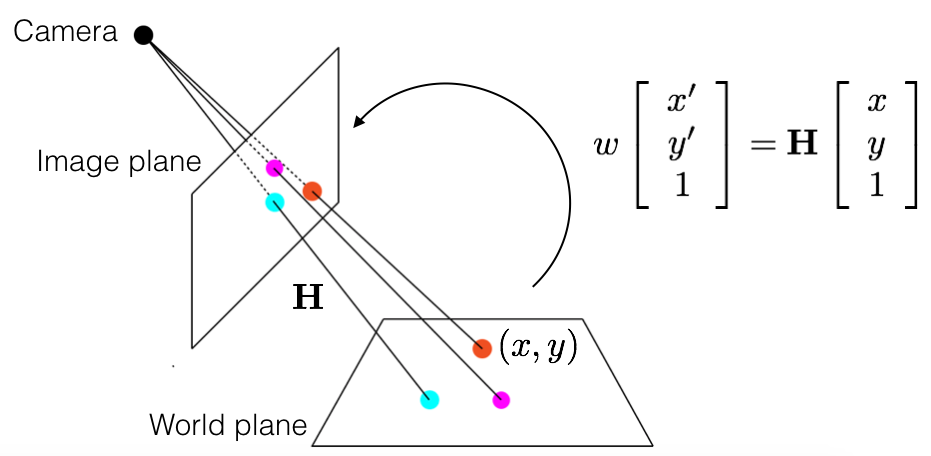
\includegraphics[width=0.6\linewidth]{homography}
\caption{Homographie, Visualisation}
\label{fig:homograpie:1}
\end{figure}
		
Die Homographie Matrix H beschreibt wie die Originalpunkte x,y zu liegen kommen in der Bildebene. Die Homographie Matrix benötigt jeweils 4 Punkte in der Quellebene und die entsprechenden 4 Punkte in der Zielebene. \\ 
		
			
\begin{figure}[H]
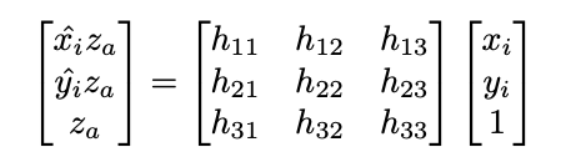
\includegraphics[width=0.6\linewidth]{homography_abbildung}
\caption{Homographie, Abbildungsgleichung}
\label{fig:homograpie:2}
\end{figure}

Wird diese Homographie Transformation in 2D gemacht, dann reicht eine 3x3 Matrix wie in Figure~\ref{fig:homograpie:2} dargestellt.
\\ In meinem Projekt werden Textures in 2D transformiert, daher reicht eigentlich eine 3x3 Matrix. \\Die 8 Punkte werden nun als Vektoren in einer Matrix A dargestellt. Die Matrixmultiplikation von A mit der Homographie Matrix die wir suchen, wird in einem Gleichungssystem von 8 Gleichungen und 8 Unbekannten gelöst.
			
			
\begin{figure}[H]
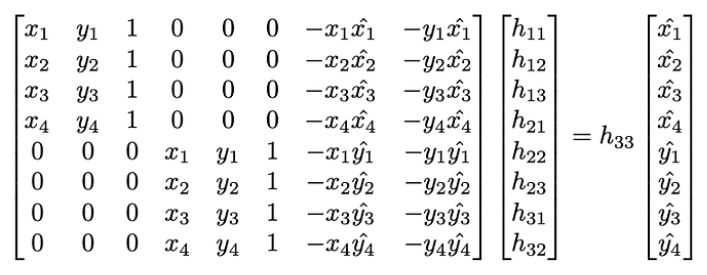
\includegraphics[width=0.6\linewidth]{homography_gleichungssystem}
\caption{Homographie, Gleichungssystem}
\label{fig:homograpie:3}
\end{figure}
		
Der Streckungsfaktor h33 zeigt, dass die Homographie Matrix noch skaliert werden kann. Im Default Fall wird h33 eins gesetzt.
\cite{OntarioTech}
\cite{HomographyEstimation}
			
\subsection{Kameramodell}


Um auf die Eckpunkte vom Screen zu kommen, sollte es reichen, wenn wir die Position der Kamera, deren Rotationswinkel, sowie den Winkel vom Field of View und den Viewport der Kamera kennen. Weiter kennen wir die World Positions von den Eckpunkten vom Screen. Da der Screen statisch ist und sich nicht bewegt, können wir dieses Model ausser acht lassen. \\ also Was bleibt sind: der Viewport (1), die Projektion (2) (Kamera intrinsisch) und das Kamera-Modell (3) (Kamera extrinsisch oder View).
Unsere Abbildungsmatrix fürs Kameramodell sieht dann so aus:
Matrix m = (1) * (2) * (3)
Und mittels Anwendung auf die Eckpunkte vom Screen:
P1' = P1 * m.
